%jsp
\section{JSP}
\subsection{概述}
\subsubsection{JSP为什么出现}
在开发web网站的时候,发现servlet做界面比较麻烦.
\begin{itemize}
\item 运行在服务器
\item 其基础是servlet(相当于对servlet的一个包装)
\item 它是一个综合技术
\begin{lstlisting}[style=JAVA]
JSP=HTML + JAVASCRIPT + JAVA CODE + JSP TAG
\end{lstlisting}
\end{itemize}


\subsubsection{JSP与SERVLET的关系}
web服务器调用jsp的过程如下图\ref{figs:fig1}所示: 
\begin{figure}[!htbp]
	\centering
	\caption{服务器调用JSP的过程}
    	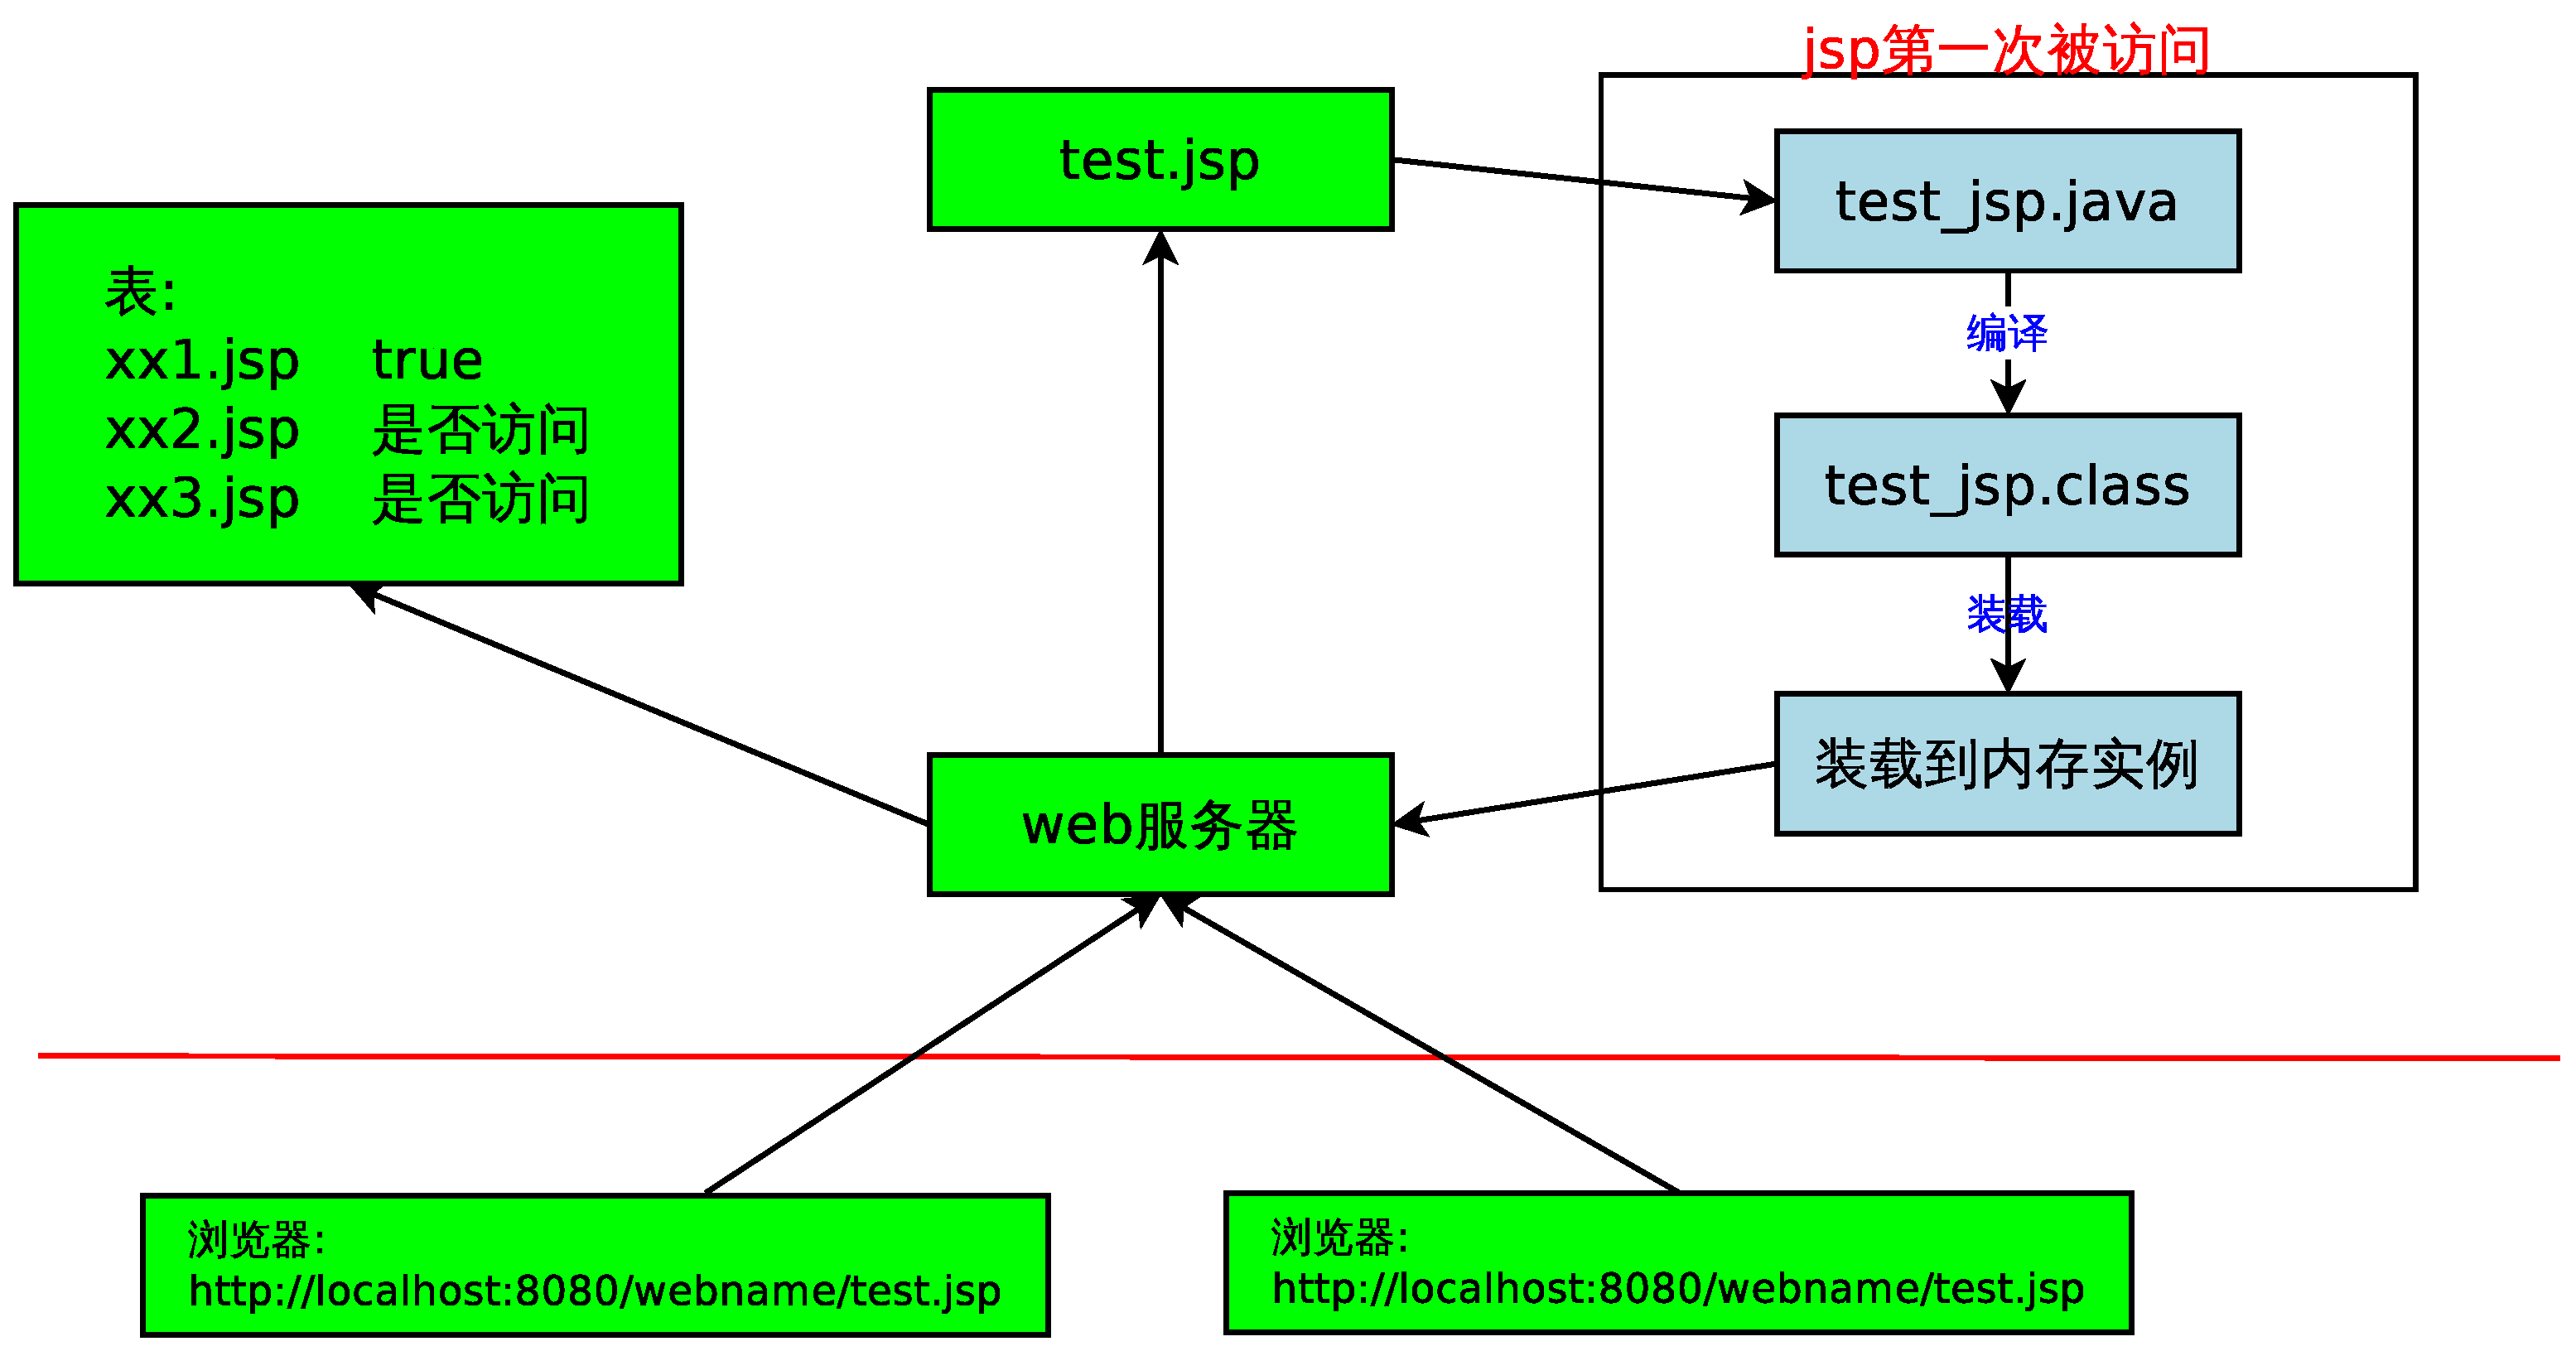
\includegraphics[scale=0.22]{figs/JSP}
    \label{figs:fig1}
\end{figure}
jsp与servlet在web应用中充当的角色如图\ref{figs:fig2}所示:
\begin{figure}[!htbp]
	\centering
	\caption{JSP与SERVLET等价}
    	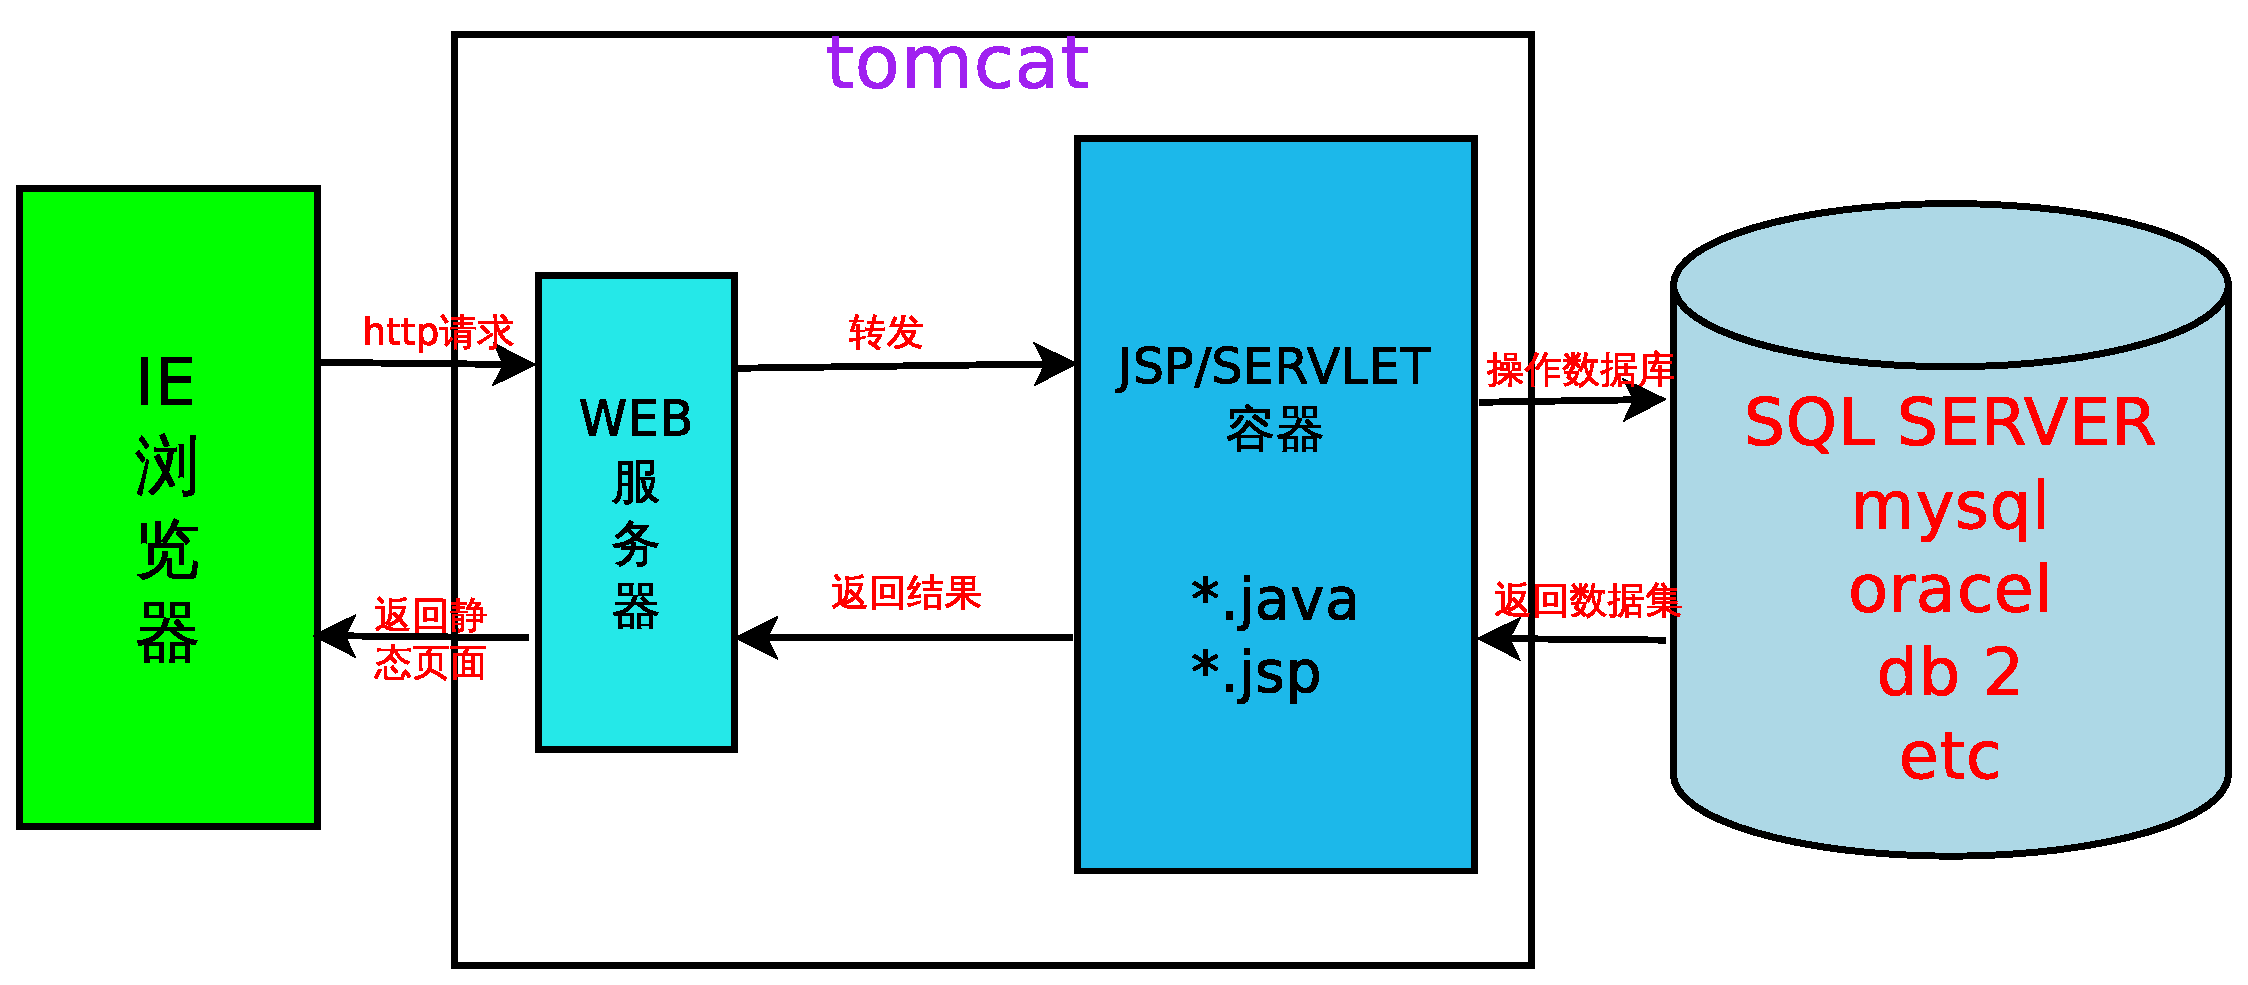
\includegraphics[scale=0.25]{figs/JSP_SERVLET}
    \label{figs:fig2}
\end{figure}
写jsp就像写html,相比只能提供静态数据的html,jsp允许在页面中嵌套java代码,为用户提供动态数据,
而相比对数据排版困难的servlet,jsp很容易实现对数据的排版.
\subsubsection{JSP标签的显示}
通过jsp九个内置对象中的out(类似servlet的PrintWriter)写入,使jsp标签发送到客户端上

\subsubsection{java代码的执行}
jsp页面中的java代码服务器直接保留,作为其内部的代码.

\subsection{语法}
\subsubsection{指令元素}
用于从jsp发送一个i信息到容器,比如设置全局变量,文字编码,引入包等.
\begin{enumerate}
\item page\\
设置jsp页面
\begin{description}
\item[contentType]	指定网页以什么方式显示页面
\item[pageEncoding]	指定servlet引擎以什么方式翻译jsp->servlet,并且指定网页以什么方式显示页面
\item[charset]	jsp页面的编码方式
\item[session]	true|false,是否禁止jsp页面中使用session会话.
\item[buffer]	none|8k|指定大小,给out对象使用的缓存区是多大.
\item[errorPage]	"相对jsp页面",如果出现错误会自动跳转到指定的页面.
\end{description}

\item include \\
引入一个jsp文件,jsp引擎会把两个jsp文件翻译成一个servlet文件.\\
\underline{被引的jsp除了保留page指令其余都删除}
\begin{description}
\item[file]	文件路径
\end{description}

\item taglib \\
自定义标签

\end{enumerate}

\subsubsection{脚本元素}
\begin{enumerate}
\item JAVA代码
\begin{lstlisting}[style=JAVA]
<%
	out.println("Hello");
%>
\end{lstlisting}
\item 表达式
\begin{lstlisting}[style=JAVA]
<%=4+5 %>
\end{lstlisting}

\item 声明
\begin{lstlisting}[style=JAVA]
<%! int i=900 //全局变量声明 %>
<%! 
	public int sum(int a,int b){ //函数声明
		return a+b;	
	}
%>
\end{lstlisting}

\end{enumerate}

\subsubsection{动作元素}
\begin{enumerate}
\item forward\\
在开发jsp的过程中,通常将jsp放入WEB-INF目录,目的是为了防止用户直接访问这些jsp文件,
在WebRoot下,有一个入口页面,主要转发
\begin{lstlisting}[style=JAVA]
<jsp:forward page="/WEB-INF/login.jsp"></jsp:forward>
\end{lstlisting}

\item include\\
\begin{lstlisting}[style=JAVA]
<jsp:include file="login.jsp"></jsp:include>
<%@ include file="login.jsp" %>
\end{lstlisting}
第一行是动态引入,第二行是静态引入,相同点都是把一个文件引入到另一个文件,区别在于
动态引入把两个jsp分别翻译,所以被引入的jsp包含有$<html><body>$,而静态引入则是把
两个jsp翻译成一个servlet,所以被引入的文件不要包含$<html><body>$.
\end{enumerate}

\subsubsection{九大内置对象}
\begin{enumerate}
\item out\\
向客户端输出数据,字节流,等价于servlet中的JspWriter

\item request\\
接受客户端的http请求,等价于servlet的HttpServletRequest
\begin{description}
\item[获取表单参数名的值]	getParameter(String name);
\item[获得表单参数名的所有值]	getParameterValues(String name);
\item[设置对应名字的值]		setAttribute(String name,Object obj);
\item[返回由name指定的属性值]	getAttribute(String name);
\item[获得cookie]	getCookie();
\end{description}

\item respones\\
封装jsp产生的回应,等价于servlet的HttpServletResponse
\begin{description}
\item[添加cookie]	addCookie(Cookie cookie);
\item[重定向]		sendRedirect("./welcome.jsp");
\end{description}


\item session\\
用于保存用户的信息,跟踪用户的行为,等价于servlet的HttpSession
\begin{description}
\item[设置属性值]	setAttribute(String name,Object obj);
\item[获得属性值]	getAttribute(String name);
\end{description}


\item application\\
多个用户共享该对象,可以做计数器,等价于servlet中的ServletContext


\item pageontext\\
代表jsp页面上的上下文,也是一个域对象,可以setAttribute(),作用范围只是本页面


\item exception\\
代表运行时的一个异常,等价于servlet中的Exception


\item page\\
代表jsp这个实例本身,等价于servlet的this


\item config
代表jsp对应的servlet的配置,等价于servlet中的ServletConfig

\end{enumerate}


\subsection{开发的模型}  
\subsubsection{纯jsp模型}



\subsection{FAQ}
